\section{Le surplus}

\subsection{Le surplus du consommateur}

On exprime le surplus du consommateur comme la quantité de ressource qu'il économise en fonction du prix du produit. 

\begin{figure}[h]
\begin{center}
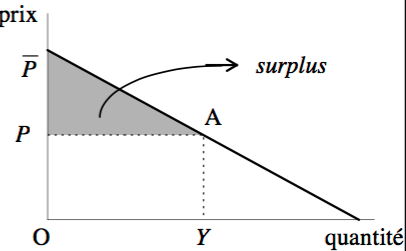
\includegraphics[scale=0.3]{./img/IM5}
\caption{Le surplus}
\end{center}
\end{figure}

Sur la figure on observe que l'individu est prêt à payer $\bar{P}$ pour une unité mais pour Y unité il paye $P^*<\bar{P}$ il réalise une économie égale à l'aire du triangle de la figure.

\subsection{Le surplus du producteur}

Dans cette section on s'intéresse en réalité au profit réalisé par le producteur. Afin de le définir on va introduire 3 notions importantes:
\begin{itemize}
\item Le coût : noté, C, il définit la fonction de cout comme la fonction qui pour un vecteur de prix donné et un niveau de production Q, donne le coût minimal. Elle est obtenue en utilisation les allocations optimales du programme de minimisation de coûts.
\item Le coût moyen : $CM=\frac{C}{Q}$
\item Le coût marginal : $C_m = \frac{\partial C}{\partial Q}$

\end{itemize}

On peut ainsi définir le profit comme $\pi = Qp - C=Qp - CM Q$ une approche graphique sur la figure suivante:


\begin{figure}[h]
\begin{center}
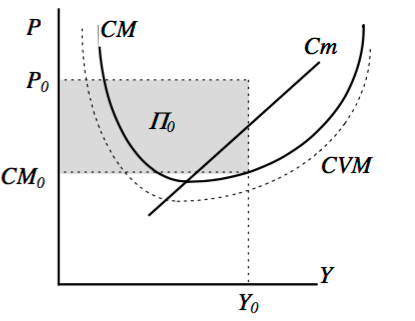
\includegraphics[scale=0.3]{./img/IM6}
\caption{Le surplus producteur avec CM}
\end{center}
\end{figure}

Ou encore avec une approche utilisant le coût marginal :
$$\pi = pQ - F - \int_0^Q$$ 
On peut remarquer qu'il y a un point que l'on nomme seuil de rentabilité, ce point est le point à partir duquel on génère du profit on le note $(p,Q^*)$ en ce point on a donc $pQ^*=CMQ=C=\int_0^{Q^*}$ on peut donc écrire:
$$\pi = pQ - F -pQ^*- \int_{Q^*}^Q$$ 
On laisse une résolution plus graphique ci-dessous.

\begin{figure}[h]
\begin{center}
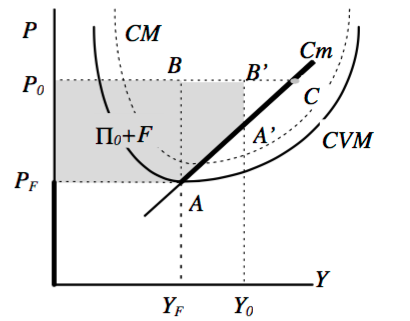
\includegraphics[scale=0.3]{./img/IM7}
\caption{Le surplus producteur avec Cm}
\end{center}
\end{figure}